\section{威胁模型与动机示例}\label{sec:threat}

本节提出一个用于系统分析事件相关攻击的威胁模型，并通过动机示例说明幻影事件的影响。
\subsection{事件交互中的信任边界}

在复杂的区块链交互环境中，建立清晰的信任边界对于全面理解交易与事件工作流中的安全风险和漏洞至关重要。\cref{fig:system model}所示的交互模型定义了三个主要信任边界：
\begin{figure}[t]
    \centering
    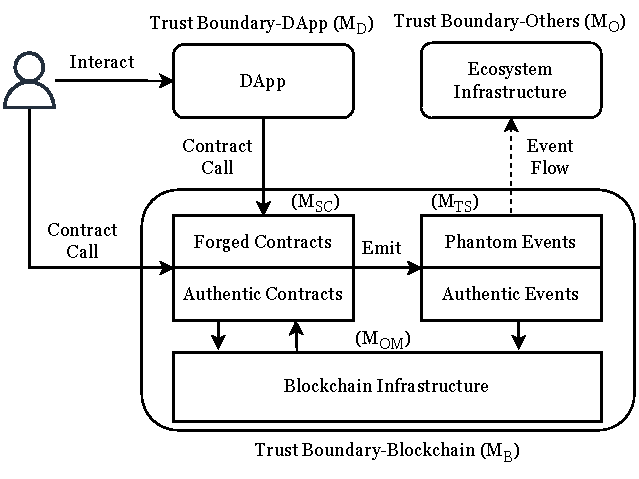
\includegraphics[width=.9\linewidth]{Sections/Picture/securitymodel.pdf}
    \caption{区块链交互中的信任边界}
    \label{fig:system model}
\end{figure}

\paragraph{信任边界-区块链（\(\bm{\mathcal{M}}_B\)）}
核心信任边界是区块链，它作为系统的基础支撑，用于存储交易和智能合约事件。
该边界内包含交易存储（\(\bm{\mathcal{M}}_{TS}\)），可进一步划分为\emph{幻影事件}和\emph{真实事件}。
幻影事件是人为创建或操纵的事件，可能触发非预期操作；真实事件则是区块链交易的预期输出。
智能合约区域（\(\bm{\mathcal{M}}_{SC}\)）可划分为\emph{真实合约}和\emph{伪造合约}，分别表示合约按预期运行或恶意运行的可能性。
其他区块链模块（\(\bm{\mathcal{M}}_{OM}\)）包括共识机制、节点通信协议以及其他支撑区块链功能的组件。

\paragraph{信任边界-DApp（\(\bm{\mathcal{M}}_{D}\)）}
第二个边界涵盖作为用户与区块链之间接口的 DApp。
DApp 会监听来自区块链的事件并作出相应响应，通常会根据这些事件触发交易或更新。


\paragraph{信任边界-其他组件（\(\bm{\mathcal{M}}_{O}\)）}
第三个边界包括更广泛的生态系统，例如链下服务、外部 API 和钱包。这些组件同样依赖区块链事件的完整性来保证其功能正常运行。

\subsection{威胁模型}
在我们的威胁模型中，攻击者试图通过发出伪造事件来破坏 DApp 及更广泛的生态基础设施，也可能利用这些攻击并结合社会工程学手段误导用户。普通用户通过调用真实合约发出合法事件，而攻击者可以通过多种方式发出伪造事件：调用伪造合约、调用真实合约，或调用一个随后再调用真实合约的伪造合约以发出伪造事件。攻击者的能力被限定为直接进行合约调用或与 DApp 交互。

\subsection{动机示例}\label{sec:motivation}
现实中已经发生了大量由交易日志伪造导致的区块链攻击。
例如，Qubit Bridge 和 pNetwork Bridge 攻击~\cite{Qubit,pNetwork}均利用了幻影事件漏洞，分别造成了 8000 万美元和 430 万美元的损失。

\begin{figure}[h]
    \centering
    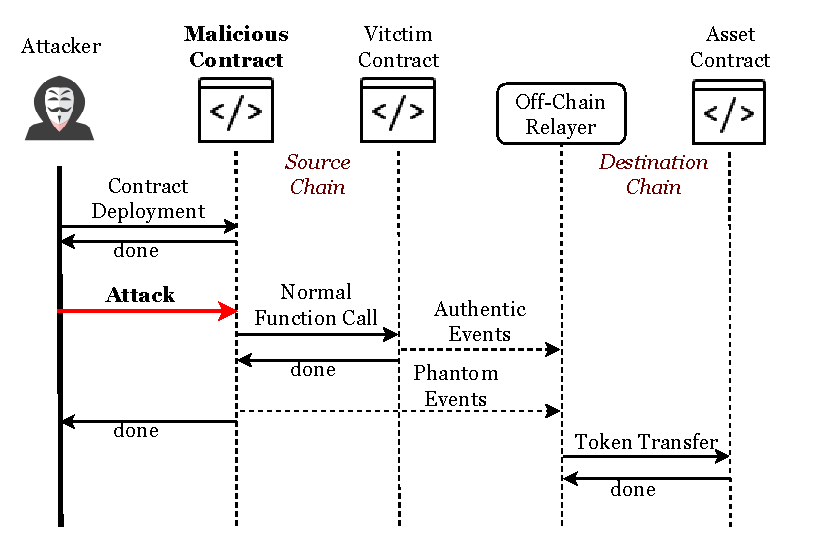
\includegraphics[width=1\columnwidth]{Sections/Picture/sequencediagram.pdf}
    \caption{pNetwork 攻击的攻击序列。}
    \label{fig:sqeuence}
\end{figure}

在 pNetwork 攻击中，事件处理机制存在缺陷：如果恶意合约和合法合约在同一笔交易中均被调用并发出事件，该机制会错误地将所有发出的事件都视为合法合约事件。因此，如攻击序列（\cref{fig:sqeuence}）所示，攻击者首先在源链上部署了恶意合约 $S_{\texttt{malicious}}$，该合约通过函数调用来调用合法合约 $S_{\texttt{legitimate}}$。在合法合约 $S_{\texttt{legitimate}}$ 执行其函数 $f_{\texttt{deposit}}$ 并发出真实事件 $E_{\texttt{Deposit}}$ 后，恶意合约 $S_{\texttt{malicious}}$ 同时发出了一个金额不真实的伪造事件 $E_{\texttt{Deposit}}$。由于真实事件和伪造事件都被记录在同一笔交易 $TX_{\textit{deposit}}$ 下，中继器便像处理合法事件一样处理了该伪造事件。攻击者由此利用系统无法区分这两个事件的缺陷，将未授权资金转移到目标链。

在 Qubit Bridge 攻击中，攻击者利用了受害合约 \texttt{deposit} 函数中的缺陷，如\cref{code:1}所示。中继器通过从源链发出的事件中获取代币地址和数量，并据此在目标链上转移资产。然而，攻击者利用 \texttt{deposit} 函数发出了本应仅由 \texttt{depositETH} 函数发出的事件，使其能够在源链上并未实际存入任何 ETH 的情况下，触发目标链上的 ETH 转账，从而绕过中继器检查并从攻击中获利。


\begin{comment}
Another example is the transfer spoofing attack on 9 February 2024, where an attacker successfully executed a \textit{transfer event spoofing} attack, resulting in a loss of \$1.04 million USD. This attack exploited vulnerabilities in wallets and blockchain explorers that parse and display transfer events. As shown in~\Cref{tab:transfer_spoof_attack_transaction}, after a user sent funds to a legitimate address (0x734\ldots{}a79F7), the attacker forged a transfer event, making it appear as though the funds were sent to a similar address controlled by the attacker. Due to the way certain wallets and explorers processed these events, the fake transfer was displayed as legitimate, leading the user to mistakenly send additional funds to the attacker's address, resulting in significant financial losses~\cite{zero_transfer}.
\end{comment}
\paragraph{\tool 的设计思路}
受这些真实案例启发，我们针对不同类型的漏洞采用了定制化检测方法。幻影事件可能源于智能合约逻辑中的问题，也可能源于链下处理器中的缺陷。为此，我们设计了一种智能合约级方法，用于识别可能导致幻影事件的漏洞。此外，我们还为交易数据开发了一种链上方法，通过检查交易中的模式或异常来判断其是否可能表明攻击。这些方法相互补充，使检测框架能够同时覆盖幻影事件中基于合约和基于交易的成因。
